\chapter{Background}
\section{Smooth Knots}

We are interested in defining a certain class of knots called Legendrian knots. Before we proceed let us give a definition for knots in general and for some of their properties, as well as touch on how we represent knots. 

\begin{definition}\label{defn:knots}
    A \textbf{knot} is a (smoothly) embedded $S^1$ in $\R^3$. Two knots are said to be \textbf{equivalent} if there exists a (smooth) isotopy of $\R^3$ taking one knot to the other.
\end{definition}
We require that knots be smooth for two reasons. The first is because non-smooth knots can be wild (pathological).
But requiring knots to be finite polygonal chains also excludes the possibility of pathological behavior, so the second reason for knots to be smooth is because further on we will define Legendrian knots using differential geometry, so our knots must be differentiable. An additional piece of information that we sometimes include with a knot is \textbf{orientation}: the "direction" that the knots runs. Knots with orientation are called \textbf{oriented}. An oriented knot has two possible orientations.

Further, define a \textbf{link} to be the union of finitely many disjoint knots. Links are a natural generalization of knots, and the knots are exactly the links with only 1 component. Links behave for the most part the same as knots. This is not always the case; for example, an oriented link with $c$ components has $2^c$ possible orientations.


We generally represent knots by \emph{diagrams}, which are projections of the knot onto a plane, marked at each double point to indicate which strand passes over the other.
Furthermore, diagrams which have no points of intersection of three or more strands, have only a finite number of double points, and in which each strand is locally flat at a double point, are called \emph{regular diagrams}. Some knot diagrams can be seen in Figure~\ref{fig:diagrams}.

\begin{figure}[ht]
    \centering
    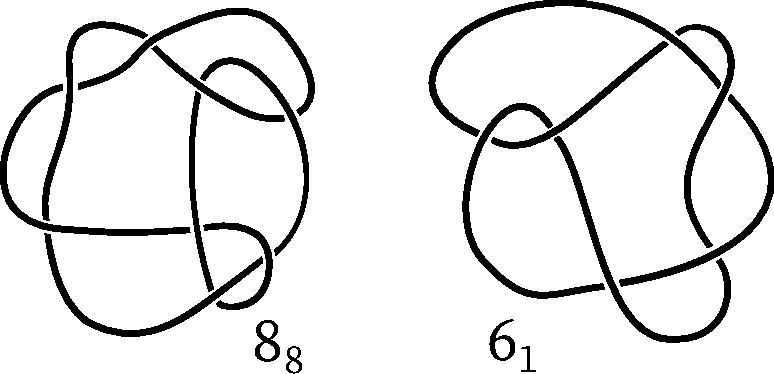
\includegraphics[width=0.45\textwidth]{images/smooth-knots.pdf}
    \caption{Knot diagrams.}
    \label{fig:diagrams}
\end{figure}

Any diagram of a tame (non-wild) knot can be approximated by a regular diagram \cite{murasugi1996}.
Moreover, regular diagrams contain enough information to reconstruct the original knot (up to isotopy). For these reasons it is very convenient to represent knots by regular diagrams, and we will make use of them here frequently. Any reference to knot diagrams should be assumed to refer to regular diagrams.

\subsection{Classification of Knots}

Given that diagrams record the entire topology of a knot, it is intuitively reasonable that we should be able to determine knot equivalence just by looking at diagrams. We are able to do so by classifying the ways that a diagram of a knot can change when the knot undergoes smooth isotopy. In particular, there are three types of diagrammatic "moves" which correspond to smooth isotopy. They are called the \textbf{Reidemeister moves}, pictured in Figure~\ref{fig:redemeister-smooth}.

\begin{figure}[ht!]
    \centering
    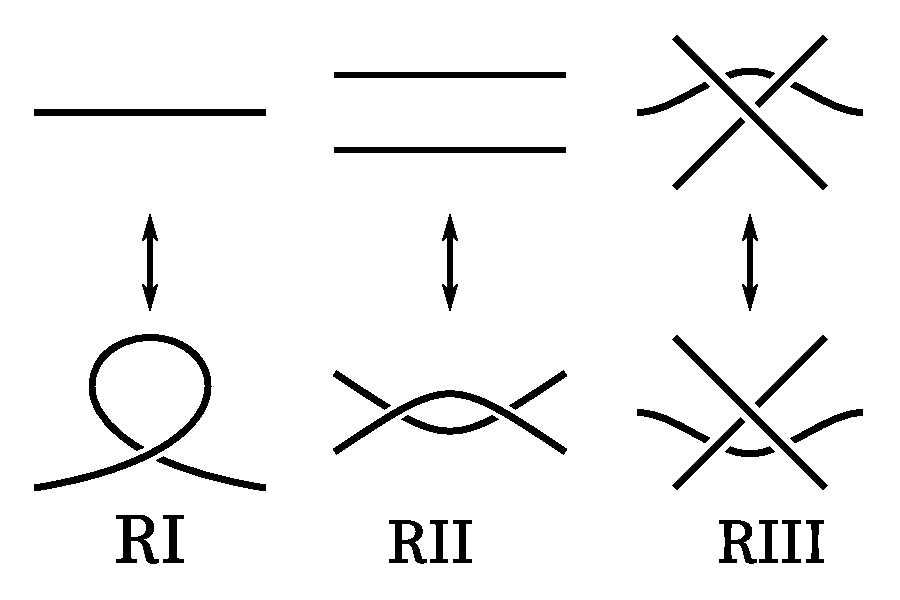
\includegraphics[width=0.5\linewidth]{images/smooth-redeimeister.pdf}
    \caption{The smooth Reidemeister moves. Reflections and rotations of these three relations are also included.}
    \label{fig:redemeister-smooth}
\end{figure}

\begin{theorem}[\cite{reidemeister}, \cite{alexander-briggs-moves}]
    Let $K$ and $K'$ be knots, with $D$ a diagram for $K$ and $D'$ a diagram for $K'$. 
    Then $K$ and $K'$ are smoothly isotopic if and only if $D$ and $D'$ are related by a finite series of Reidemeister moves (Figure~\ref{fig:redemeister-smooth}) and planar isotopy.
\end{theorem}

% TODO: Cite this
The Reidemeister moves completely determine smooth isotopy. That is, two knots $K$ and $K'$ are isotopic exactly when a diagram for $K$ can be transformed into a diagram for $K'$ by using the Reidemeister moves and planar isotopy. It remains difficult in practice to determine when two knots are equivalent. 

Since the origins of historical interest in knot theory, an ongoing project has been to create a complete table of (small) knots. There are two important simplifications we can make to reduce the number of distinct knots required for such an atlas.

First, given two knots, we can construct a new knot by splicing them together. This construction is called a connected sum, and the connected sum of $K$ and $L$ is written $K \# L$. The connected sum is well-defined, as it is topologically invariant with respect to how $K$ and $L$ are spliced.
The properties of a connected sum such as $K \# L$ can usually be determined based on knowledge about $K$ and $L$. Thus it suffices to catalogue the knots which are not connected sums; these are called \textbf{prime} knots.

Second, we can construct a new knot by changing the crossings of a diagram. In particular, given a diagram $D$ for a knot $K$, we can construct a new diagram $m(D)$ by switching the overstrand and the understrand at each crossing. Then there exists some new knot $K'$ for which $m(D)$ is a regular diagram. The resulting knot $K'$ is independent of the choice of $D$, and it is referred to as the \textbf{mirror} of $K$, or $m(K)$. Note that $m(m(K)) = K$. We say that $K$ is \textbf{amphichiral} if $m(K) = K$, but this is not the case in general. For example, the trefoil and its mirror, shown in Figure~\ref{fig:mirror}, are not equivalent.

% Maybe cite this?
\begin{figure}[ht]
    \centering
    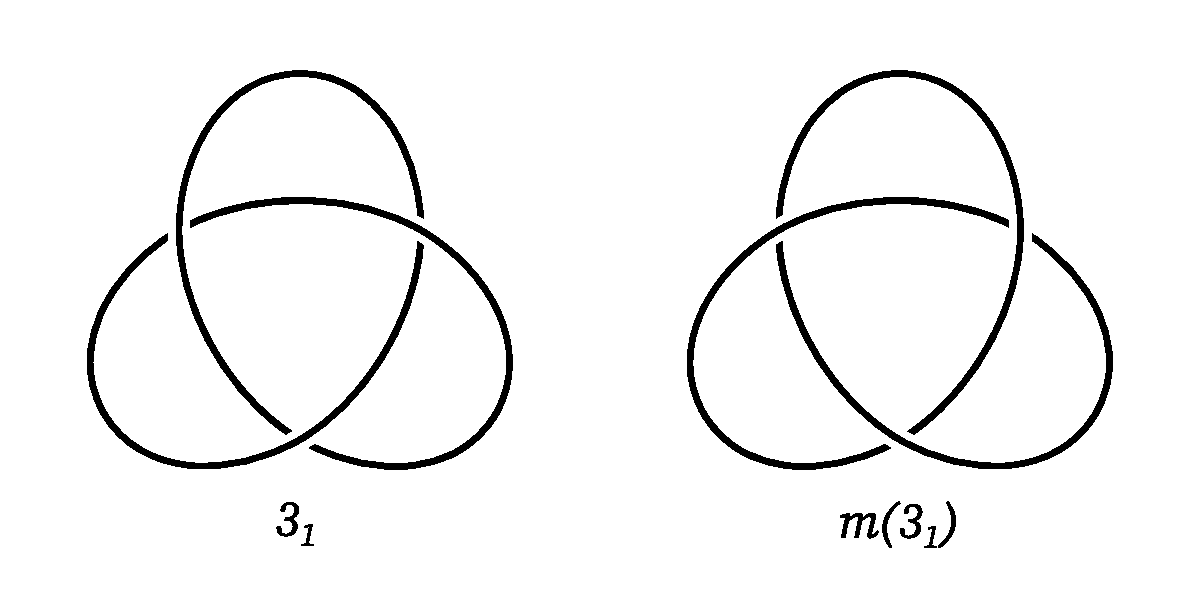
\includegraphics[width=0.5\linewidth]{images/mirror.pdf}
    \caption{The left-handed trefoil $6_1$ and the right-handed trefoil $m(6_1)$.}%
    \label{fig:mirror}
\end{figure}

Such tables are organized according to the \textbf{crossing number}, which is defined for a knot $K$ as the minimum number of crossings over all regular diagrams of $K$.
There are finitely many prime knots of a given crossing number, and within tables they are ordered arbitrarily (although there is an agreed-upon numbering of prime knots up to 10 crossings) and numbered. For more information on knot tables, see \cite{hoste}.

For example, a reference to the knot $6_1$ as in Figure~\ref{fig:diagrams} should be read as the \emph{1st} prime knot with a crossing number of \emph{6}. This is called \textbf{Alexander-Briggs notation}, named for and following the convention of an important early knot table \cite{alexander-briggs}.

\section{Legendrian Knots}
\subsection{Contact Geometry}

In order to define Legendrian knots we begin by defining a certain plane field on $\R^3$; it is called the \textbf{standard contact structure}, or $\xi$ (Figure~\ref{fig:contact-planes}). At each $(x, y, z) \in \R^3$ we define
\[
    \xi(x, y, z) = \lspan \{\partial_y, \partial_x + y\partial_z\}.
\]

Note that $\xi$ is defined as a linear combination of the partial derivatives of the coordinate functions, as these are the basis vectors of the tangent space $\tpm_{(x, y, z)} \R^3$, of which $\xi$ is a 2-dimensional subspace.

Every plane field is the kernel of a 1-form. In the case of the standard contact planes $\xi$, this one form is referred to as $\alpha_0$, and it is given by ${\alpha_0 = dz - y \, dx}$.

\begin{figure}[ht]
    \centering
    % Yes I squashed the aspect ratio. I think the proportions of the original are ugly!
    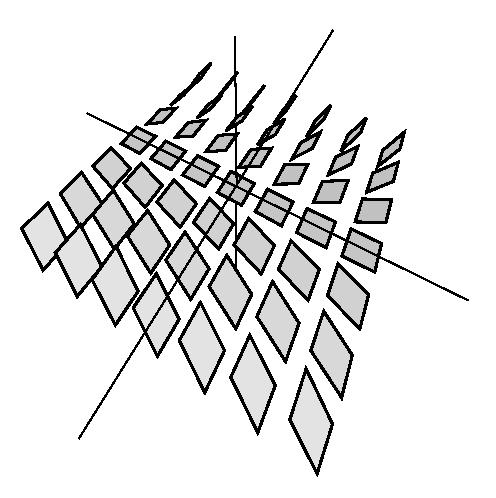
\includegraphics[width=0.6\textwidth, height=2.6in]{images/contact-planes.pdf}
    \caption{The standard contact planes in $\R^3$. Diagram from S. Schonenberger.}%
    \label{fig:contact-planes}
\end{figure}

As we go along the $y$-axis, the plane $\xi(p)$  gets steeper and steeper in the $\partial x$ direction. In fact, the planes twist so much that there is no 2-dimensional surface everywhere tangent to $\xi$, or even tangent to $\xi$ in any open set \cite{boothby}.
% Maybe show the proof with the lie bracket...
Such a plane field is called \textbf{completely non-integrable}.
In general, a 3-manifold equipped with a completely non-integrable plane field is called a \textbf{contact 3-manifold}.

Although no surface can be everywhere tangent to $\xi$, there are many curves which run tangent to $\xi$. Such a curve is called Legendrian, leading to the following definition.

\begin{definition}
    Let $K: (0, 1) \to \R^3$ be a smooth curve. We say $K$ is \textbf{Legendrian} if $K$ is everywhere tangent to $\xi$. That is, at all $t \in (0, 1)$,
    \[
        K'(t) \in \xi(K(t)).
    \]
\end{definition}

As a knot is a smooth embedding of the circle in $\R^3$, so a Legendrian knot is a Legendrian embedding of the circle in $(\R^3, \xi)$. But the equivalence relation under which one defines a knot is as important as the curve itself, and so we will define an analogous relation for Legendrian knots. 

\begin{definition}
    Let $K$ and $K'$ be Legendrian knots. We say $K$ and $K'$ are \textbf{Legendrian equivalent} if there exists a smooth function ${\phi: [0, 1] \to \R^3}$ such that
    ${\phi(0) = K}$, ${\phi(1) = K'}$, and for any ${t \in [0, 1]}$, $\phi(t)$ is a Legendrian knot.
\end{definition}

The only difference between this definition and Definition \ref{defn:knots} is that the intermediate knots must also be Legendrian.
We frequently use the terms \textbf{equivalent} and \textbf{isotopic} to refer to knots that are either Legendrian equivalent or smoothly equivalent. Generally, when referring to Legendrian knots, we mean Legendrian equivalence, but when confusion may arise we will explicitly use the term \textbf{smoothly equivalent/isotopic}.

By definition, all Legendrian knots are smooth knots, and it is clear that there are representatives of smooth knots which are not Legendrian. Nonetheless, Legendrian knots are plentiful. In fact, any knot can be $C^0$ approximated by a Legendrian knot (a proof of this fact will be given in Section~\ref{subsec:invariants}, once we have defined stabilization).
% TODO: put in this proof 
Such an approximation is smoothly isotopic to the target curve, and thus there exist Legendrian representatives of any smooth knot type.

\subsection{Front Diagrams}

Representatives of Legendrian knots are no different from smooth knots, in that they are embeddings of $S^1$ in $\R^3$, and so it is convenient to represent them by diagrams.

Unlike smooth knots, Legendrian knots contain geometric information, and so we want our diagrams to record that information too. But because the geometric condition that Legendrian knots satisfy is not invariant under rotation, we must be careful to distinguish which plane we are projecting onto to create a diagram.

There are two projections which are used to represent Legendrian knots. The first is the Lagrangian diagram, which is projection onto the $xy$ plane. This projection is useful in defining certain algebraic invariants, but we will not need it here.
% Awk!
Instead, we restrict our examination to the \textbf{front projection}, which is projection onto the $xz$ plane such that the positive $y$ direction points \emph{into} the page. This orientation agrees with the right-hand rule: the positive $x$ direction points to the east, the positive $z$ direction points north, and then the right-hand rule tells us that the positive $y$ direction points into the page.

\begin{figure}[ht]
    \centering
    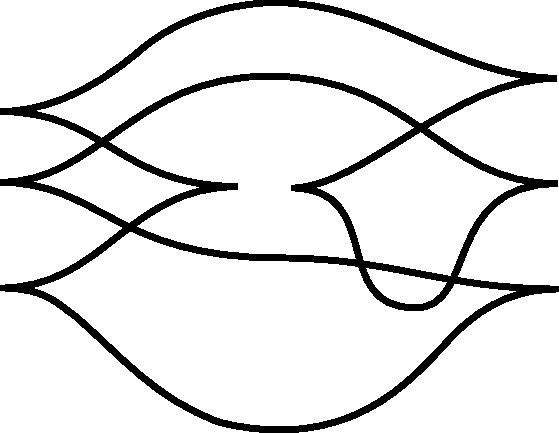
\includegraphics[width=0.3\textwidth]{images/chekanov-1.pdf}
    \hspace{2em}
    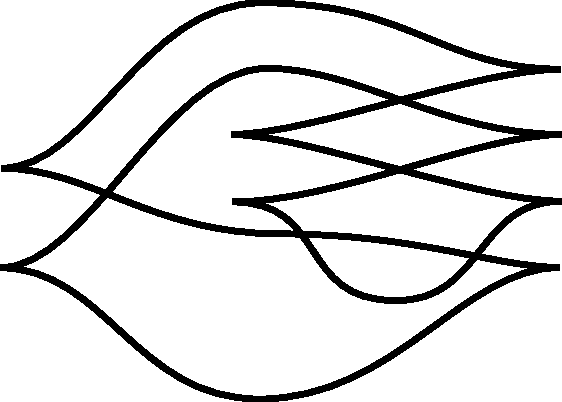
\includegraphics[width=0.3\textwidth]{images/chekanov-2.pdf}
    \caption{Front projections for some Legendrian knots (the Chekanov examples).}%
    \label{fig:front-projection}
\end{figure}

Front projections, Figure~\ref{fig:front-projection}, contain enough information to recover the exact geometry of the original knot. This is because the Legendrian condition is a requirement on the tangent vector based on the $y$-coordinate. Recall that a curve $K$ is Legendrian if ${\alpha = dz - y\, dx}$ vanishes on $\tpm_p K$ for all $p \in K$. Thus we have ${dz - y \, dx = 0}$ and so
\[
    y = \frac{dz}{dx}.
\]
This explains the cusps we see on the left and right sides of front diagrams: Since the part above the cusp (which has a negative slope, in the case of a right cusp) and the part below the cusp (which has a positive slope at a right cusp) have to meet, the slopes of each must be equal at the cusp. Note that while these points are cusps in the projection, they are smooth in the 3-dimensional knot.

Moreover, in a front diagram there is no need to mark the overstrand at a crossing: unambiguously, the strand with a more negative slope goes over the other.

One other way that we represent Legendrian knots is with \textbf{grid diagrams}. Grid diagrams are composed of axis-alined line segments on an integer grid with all the overstrands vertical.
A grid diagram for the knot $5_2$ is shown in Figure~\ref{fig:grid}.
A front diagram may be obtained from a grid diagram by rotating the figure $45^\circ$ counterclockwise (such that the overstrands run diagonally down), smoothing out the up and down corners, and sharpening the left and right corners into cusps. Similarly, a grid diagram can be obtained from a front diagram. 

\begin{figure}[ht]
    \centering
    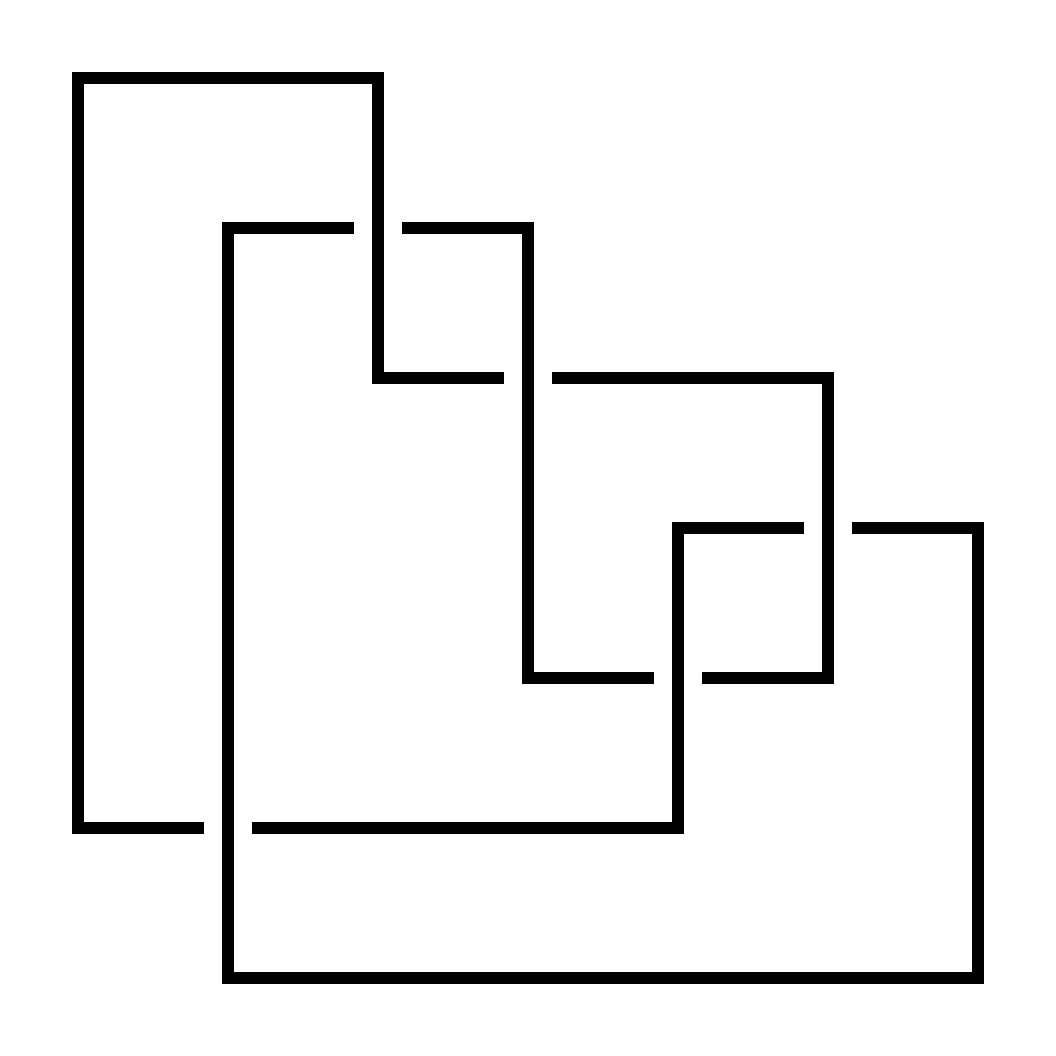
\includegraphics[width=0.3\textwidth]{images/5_2-grid.pdf}
    \label{fig:grid}
    \caption{A grid diagram for the knot $5_2$.}
\end{figure}

Often, grid diagrams are defined to include the requirement that each column or row of the grid contains exactly one segment --- that is, there are no disjoint collinear segments; such diagrams are also referred to as \textbf{arc diagrams}. This form makes grid diagrams a convenient way of representing Legendrian knots in computer programs, as it suffices to supply the coordinates of the corners. Since there are no disjoint collinear segments, each corner point shares a row with exactly one other point and a column with exactly one other. The knot can be drawn by connecting these corners, with the vertical strands running over the horizontal strands.


\subsection{Classical Invariants}\label{subsec:invariants}

Any two knots which are Legendrian equivalent are also smoothly equivalent by definition, so let us ask whether the converse is true.
As you may expect the answer is no. Moreover, since we can approximate any smooth knot by an isotopic Legendrian one, the relation of Legendrian equivalence ``refines'' the equivalence classes of smooth knots into a larger number of Legendrian equivalence classes. What does the structure of this refinement look like? As expected this is a nontrivial question. We will begin to answer it by looking at equivalence of diagrams.

We saw earlier that the equivalence of smooth knots corresponds to equivalence of diagrams under the Reidemeister moves. The Reidemeister moves do not preserve Legendrian equivalence, but there exists a similar set of three diagrammatic moves, Figure~\ref{fig:redemeister}, which determine Legendrian equivalence of front diagrams.

\begin{figure}[ht]
    \centering
    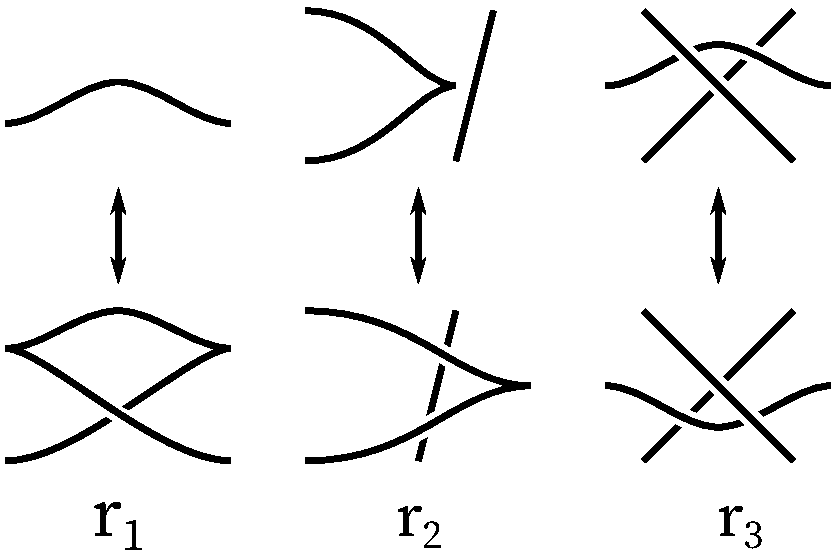
\includegraphics[width=0.5\textwidth]{images/redeimeister.pdf}
    \caption{The Legendrian Reidemeister moves. Vertical and horizontal reflections of these moves are also allowed, as long as the crossings are corrected so that the overstrand has the more negative slope.}%
    \label{fig:redemeister}
\end{figure}

\begin{theorem}[\cite{swiatkowski}]
    Let $K$ and $K'$ be Legendrian knots, with $D$ a front diagram for $K$ and $D'$ a front diagram for $K'$.
    Then $K$ and $K'$ are Legendrian isotopic if and only if $D$ and $D'$ are related by a finite sequence of Legendrian Reidemeister moves (Figure~\ref{fig:redemeister}) and planar isotopy.
\end{theorem}

These moves correspond to restricted versions of the smooth Reidemeister moves.
Unfortunately, as with the smooth Reidemeister moves, it is difficult in practice to determine equivalence of knots using these rules. Nonetheless, they are useful in the construction of more practical invariants, as invariance under all three Reidemeister moves is equivalent to invariance under Legendrian isotopy.


There are two numerical invariants which can be easily defined in and computed from the front projection, and they are called the \textbf{classical invariants}. Before we define them, we need to define the \textbf{writhe} of a diagram.

To define the writhe $w(D)$ of a diagram $D$, we assign a sign to each crossing in $D$, using the right-hand rule as seen in Figure \ref{fig:writhe}. If as you travel along the overstrand, the understrand goes from right to left, then the crossing is positive; and if the understrand runs from left to right then the crossing is negative. 
The writhe is the sum of the signs of the crossings.

\begin{figure}[ht]
    \centering
    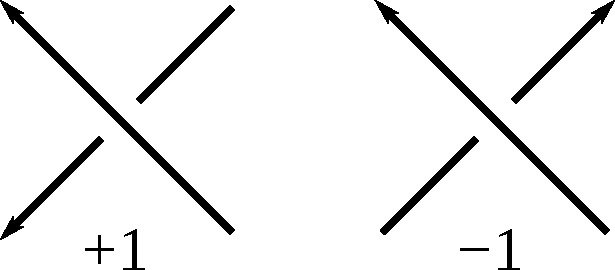
\includegraphics[width=0.7\textwidth]{images/writhe.pdf}
    \caption{The sign at a crossing.}%
    \label{fig:writhe}
\end{figure}

Writhe is \emph{not} an invariant of Legendrian knots. Because the RI move adds a crossing without changing the orientation of other crossings, it changes the writhe. But it allows us to define the following invariant.

\begin{definition}
    Let $K$ be a Legendrian knot, and $D$ a front diagram for $K$. Let $\cusps_r(D)$ be the number of right cusps in $D$, and $w(D)$ the writhe of $D$.
    Define the \textbf{Thurston-Bennequin number}, or $\tb$, as
    \[
        \tb(K) = w(D) - \cusps_r(D).
    \]
\end{definition}

It is a simple matter to show that the Thurston-Bennequin number is an invariant of Legendrian knots.

\begin{proposition}
    The Thurston-Bennequin number is an invariant of Legendrian knots.
\end{proposition}
\begin{proof}
    Let $D$ be a front diagram for a Legendrian knot $K$. It suffices to show that $\tb(D)$ is unchanged under the Legendrian Reidemeister moves.

    \begin{enumerate}
        \item RI adds one right cusp and one crossing. Regardless of the orientation of the segment before the move, the new crossing is easily seen to have sign $+1$, and therefore
            \[
                \tb(D') = (w(D) + 1) - (\cusps_r(D) + 1) = \tb(D).
            \]
        \item RII adds two crossings, but they have opposite signs, so the writhe remains the same.
        \item RIII moves two crossings, but their signs remain unchanged.
    \end{enumerate}
    
\end{proof}

\begin{definition}
    Let $K$ be a Legendrian knot and $D$ a front diagram for $K$.
    Given an orientation ($t$ increasing), we say a cusp is \emph{upward-pointing} (resp. \emph{downward}) if $\frac{dz}{dt} > 0$ near the cusp (resp. $< 0$).
    Let $\cusps_u(D)$ be the number of upward-pointing cusps and $\cusps_d(D)$ be the number of downward-pointing cusps. Define the \textbf{rotation number} of $K$ as 
    \[
        \rot(K) = \frac{1}{2} (\cusps_d(D) - \cusps_u(D)).
    \]
    Although $\rot(K)$ is only well-defined for \emph{oriented} $K$, it is defined up to multiplication by $\pm 1$ for unoriented knots.
\end{definition}
\begin{proposition}
    The rotation number is an invariant of Legendrian knots.
\end{proposition}
\begin{proof}
    As before, we show that $\rot(K)$ is an invariant, so let $D$ be a front diagram for $K$. Neither RII nor RIII change the orientation or the number of cusps. On the other hand, RI creates a pair of cusps, one pointing upward and one pointing downward.
\end{proof}

These invariants do a good job of distinguishing Legendrian knots (see \cite{eliashberg2008unknot}), though there are known to be pairs of smoothly-isotopic Legendrian knots which have the same $\tb$ and rotation number but which are not Legendrian equivalent (Figure~\ref{fig:front-projection}, \cite{chekanov}). But the existence of these invariants reveals a great deal about how the Legendrian equivalence classes of a smooth knot are structured. 

\begin{figure}[ht]
    \centering
    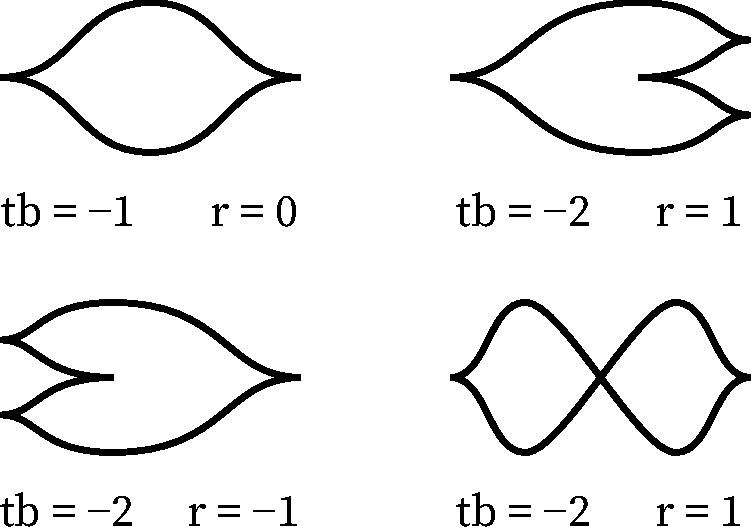
\includegraphics[width=0.4\textwidth]{images/unknots.pdf}
    \caption{A selection of Legendrian unknots.}%
    \label{fig:unknots}
\end{figure}

% Awk
Figure~\ref{fig:unknots} shows four Legendrian unknots. The top left has $\tb = -1$ and the others have $\tb = -2$, so the first is not isotopic to the rest. But the unknots with $\tb = -2$ can be obtained from the first by means of a so-called \textbf{stabilization}, shown in Figure~\ref{fig:stabilization}. 

\begin{figure}[ht]
    \centering
    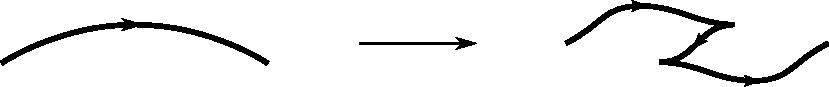
\includegraphics[width=0.6\linewidth]{images/stabilization.pdf}
    \caption{A ``positive'' stabilization, increasing the rotation number.}%
    \label{fig:stabilization}
\end{figure}

% Do you need to explicitly mention that stabilization preserves smooth knot type?
A stabilization decreases the $\tb$ by 1, and changes the rotation number by $\pm 1$ depending on the orientation. Thus for any topological knot, the $\tb$s of its Legendrian representatives are unbounded below, and the rotation numbers are unbounded both above and below.

% Add a proof of C^0 approximation

It is known that for any topological knot, the $\tb$ is bounded above \cite{bennequin}, and therefore the \textbf{maximal Thurston-Bennequin number} is a knot invariant, which we denote $\maxtb(K)$.
For example, the maximal $\tb$ for the unknot is $-1$, as seen in Figure~\ref{fig:unknots}, and all other representatives are (Legendrian isotopic to) stabilizations of the maximal-$tb$ unknot \cite{atlas}. It is possible to determine whether a Legendrian knot is a stabilization using the Chekanov-Eliashberg DGA, but this does not in general determine $\maxtb$: there exists a Legendrian representative of $m(10_{139})$ with $\tb = -17$ and $\rot = 4$ which is not a stabilization of the maximal-tb representative, which has $\tb = -16$ and $\rot = 1$. Thus we have to look elsewhere to determine $\maxtb$.

\subsection{Polynomial Invariants and Skein Relations}

Many useful knot invariants take the form of Laurent polynomials (i.e., having both positive and negative exponents). Typically, these are defined recursively using skein relations, which give an algebraic relationship between the polynomials of knots differing only at a crossing. For certain such relations the resulting polynomial can be shown to be not only unique, but invariant under isotopy.

In particular, we are interested in the Kauffman polynomial, as it gives an upper bound on the maximal $\tb$ of a smooth knot type. We define the Kauffman polynomial in terms of the L-polynomial, which is an invariant only under regular isotopy.
There are many varying definitions of the Kauffman polynomial in the literature. We use here a variant known as the \textbf{Dubrovnik polynomial} (it was discovered in the city of Dubrovnik in then-Yugoslavia \cite{kauffman}), and we refer to its normalized version as the \textbf{Kauffman polynomial}. 
It is known that the Dubrovnik polynomial and other formulations of the Kauffman polynomial are interconvertible \cite{kauffman}.
Our formulation matches that used by \cite{ferrand} and is similar to that used by \cite{lu-zhong}. See Appendix \ref{chap:appendix} for details on their version.

Let $T$ be a knot diagram or an oriented link diagram, and define the \textbf{Dubrovnik Polynomial} $D$ recursively via the following skein relations, where ${\delta = \frac{a - a^{-1}}{z} + 1}$.
\begin{align}
    D\left(\Lmin\right) - D\left(\Lplus\right) &= z \left( D\left(\Lzero\right) - D\left(\Linf\right) \right) \\
    D\left(\Lr\right) &= a D \Big(\Ln\Big)\\
    D\left(\Lu\right) &= \delta
\end{align}

The first two equations are local, indicating a relation between the Dubrovnik polynomials of diagrams which are identical except for the substitution of the indicated figures. The third equation normalizes the recurrence relation by determining the Dubrovnik polynomial of an unknot diagram without crossings. The choice of $\delta$ for the polynomial of the unknot is natural; it arises from setting $D(\emptyset) = 1$ for the empty link.

Yet such a polynomial is certainly not a topological invariant: the RI move corresponds to multiplication by $a^{\pm 1}$. Thus we normalize the D-polynomial by the writhe to get the Kauffman polynomial $Y(K)$, since the same RI move which corresponds to a multiplication by $a$ in the Dubrovnik polynomial increases the writhe by 1. This is why we require that $K$ be oriented if it is a link and not a knot: writhe is well-defined for unoriented knots but not for unoriented links in general.
\begin{definition}
    Let $K$ be a knot or an oriented link and $T$ a diagram for $K$. Define the \textbf{Kauffman Polynomial} of $K$ by
    \[
        Y(K) = a^{-w(T)} D(T).
    \]
    The polynomial, which is a Laurent polynomial in $a, x$, is an invariant under smooth isotopy \cite{kauffman}.
\end{definition}

As an example, we show here the computation of the Kauffman polynomial of the trefoil.

The degree of the framing variable $a$ in the Kauffman polynomial gives rise to an upper bound on the $\tb$, which was first proved by Rudolph \cite{rudolph}. The version we use here is due to Tabachnikov \cite{tabachnikov}. More information on this bound and its history can be found in \cite{ferrand}.

\begin{theorem}[Kauffman Bound \cite{tabachnikov}]\label{kauffman-bound}
    If $K$ is a Legendrian link, then $\overline{tb}(K) \leq \mu_a(Y(K))$, where $\mu_a(P)$ denotes the minimum degree of $a$ in the polynomial $P(a, x)$.
\end{theorem}

This bound is very useful: there is no method in general for computing the maximal $\tb$ of a knot, but it is a fairly straightforward matter to compute its Kauffman polynomial. The bound fails to be sharp in some known cases (e.g., \cite{ferrand}) but there are also classes of knots for which it is known to be sharp. These include positive knots, most torus knots, 2-bridge links, and most 3-twist pretzel links. That the Kauffman bound is sharp for many 3-twist pretzel links is a theorem of Ng:

\begin{theorem}[\cite{ng}]
    Suppose $p_1, p_2, p_3 > 0$. Then the Kauffman bound is sharp for the pretzel links $P(p_1, p_2, p_3)$, $P(-p_1, p_2, p_3)$, and $P(-p_1, -p_2, -p_3)$, and for $P(-p_1, -p_2, p_3)$ when $p_1 \geq p_2 \neq p_3 + 1$.
\end{theorem}

We will make use of this theorem in our main result.

\section{Lagrangian Cobordisms}

\subsection{Symplectic Geometry}

Cobordisms are objects originating in smooth knot theory --- in essence, surfaces having specific knots as boundary --- which define a fundamental relation between types of knots. We define them here in the context of smooth knots, and then we will be able to define a type of cobordism called a Lagrangian cobordism by requiring that it be everywhere tangent to a certain differential form.

\begin{definition}
    Let $K$ and $K'$ be smooth knots. Define a \textbf{cobordism} as a smoothly embedded 2-manifold with boundary $A$ in $\R^3 \times I$ such that the ``bottom'' ($t = 0$) edge of $A$ is $K$ and the ``top'' ($t=1$) edge of $A$ is $K'$. That is,
    \begin{align*}
        A \cap \left(\R^3 \times \{0\}\right) &= K \times \{0\}\\
        A \cap \left(\R^3 \times \{1\}\right) &= K' \times \{1\}
    \end{align*}
\end{definition}

We extend this definition by defining a \textbf{symplectic manifold} in much the same way we defined a contact manifold: as a manifold equipped with an appropriate differential form. Recall that a 2-form $\omega$ on a manifold $X$ is \textbf{closed} if $d \omega = 0$ (i.e., its exterior derivative vanishes) and \textbf{nondegenerate} if for any $\vec v \neq 0$, ${\omega(\vec v, \vec w) \neq 0}$ for all ${\vec w \in \tpm_p X}$.

\begin{definition}
    Let $X$ be a 4-dimensional smooth manifold and $\omega$ a 2-form on $X$ that is closed and nondegenerate. Then the pair $(X, \omega)$ is said to be a \textbf{symplectic 4-manifold}.
\end{definition}

Analogous to Legendrian curves in contact manifolds are Lagrangian surfaces in symplectic manifolds.
\begin{definition}
    Let $(X, \omega)$ be a symplectic 4-manifold and $L$ a smoothly embedded 2-manifold in $X$. We say $L$ is \textbf{Lagrangian} if for all $p \in L$, $\omega$ vanishes on $\tpm_p L$.
\end{definition}

% This section could do with a rework -- either go more into depth or less into depth.

% give a citation for this
Given a contact manifold $(Y, \ker \alpha)$ there is a canonically associated symplectic manifold $(Y \times \R, d(e^t \alpha))$, where $t$ is the coordinate on the attached copy of $\R$. This allows us to put Legendrian knots into symplectic manifolds as slices of Lagrangian submanifolds. Thus a Lagrangian cobordism is a Lagrangian surface that is also a cobordism, with a few extra conditions required.

\begin{definition}
    Let $K_-$ and $K_+$ be Legendrian links, and $L$ a (orientable, exact) Lagrangian manifold in $(\R^3 \times \R, d(e^t \alpha))$. We say $L$ is a \textbf{Lagrangian cobordism} from $K_-$ to $K_+$ if for some $T > 0$,
    \begin{align*}
        L \cap \left(\R^3 \times (-\infty, -T)\right) &= K_- \times (-\infty, -T)\\
        L \cap \left(\R^3 \times (T, \infty)\right) &= K_+ \times (T, \infty)\\
        L \cap \left(\R^3 \times [-T, T] \right)\, &\,\, \text{is compact}
    \end{align*}
    and there exists a function $f: L \to \R$ such that ${df = e^t \alpha |_{\tpm L}}$ and $f$ is constant for $t \geq T$ and $t \leq -T$.

    We call a $L$ a \textbf{concordance} if $K_-$ and $K_+$ are knots and $L$ has genus zero.

\end{definition}

\begin{figure}[ht]
    \centering
    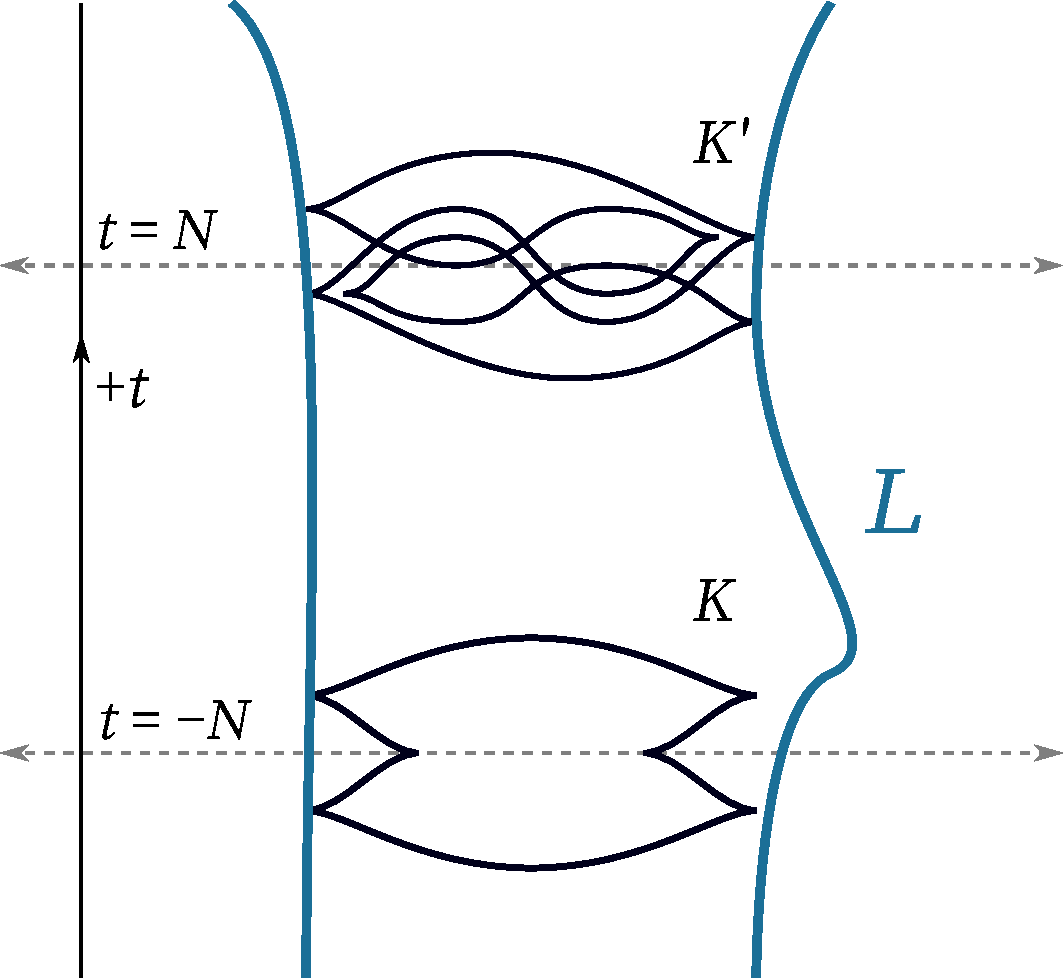
\includegraphics[width=0.5\textwidth]{images/cobordism-visualization.pdf}
    \caption{A visualization of a Lagrangian cobordism $L$ as an infinite cylinder which looks like $K_-$ for $t \leq -N$ and $K_+$ for $t \geq N$. Each slice along the $t$ axis is an entire $\R^3$. In this diagram $K_-$ is the unknot and $K_+$ is $m(6_1)$.}%
    \label{fig:cobordism-vis}
\end{figure}

Smooth cobordisms have boundary, and the knots $K_-$ and $K_+$ together form that boundary. Lagrangian cobordisms do not have boundary: rather, we think of the cobordism as ``looking like'' the knots below and above some $t$-value, respectively.
But this difference is largely inconsequential.
More importantly, we have added an asymmetric geometric condition on the cobordism, and the result is that the relation "there exists a Lagrangian cobordism from $K_-$ to $K_+$" is not symmetric \cite{chantraine2015}.

We make the distinction between cobordisms with genus and concordances because the genus of a cobordism gives a lot of information about the two knots at its ends \cite{chantraine2010}. In particular, if $L$ is a cobordism from $K_-$ to $K_+$,
\[
    \rot(K_-) = \rot(K_+) \text{     and     } \tb(K_+) - \tb(K_-) = 2g(L).
\]
Thus a Lagrangian concordance can only exist between two knots with equal rotation number and $\tb$.


\subsection{Constructable cobordisms}

In general, Lagrangian cobordisms are difficult to find. However, there are several conditions in which they are known to exist. Of interest is a certain set of moves which may be easily defined on front diagrams, the Reidemeister moves among them, such that a Langrangian cobordism exists between knots related by them.

\begin{theorem}[\cite{bourgeois15}]
    Suppose $K_-$ and $K_+$ are Legendrian knots. If the front diagram of $K_+$ can be obtained from the front diagram of $K_-$ by a finite sequence of handle moves (Figure~\ref{fig:handles}), Legendrian Reidemeister moves (Figure~\ref{fig:redemeister}), and planar isotopy, then there exists a Lagrangian cobordism from $K_-$ to $K_+$. 
\end{theorem}
\begin{figure}[ht!]
    \centering
    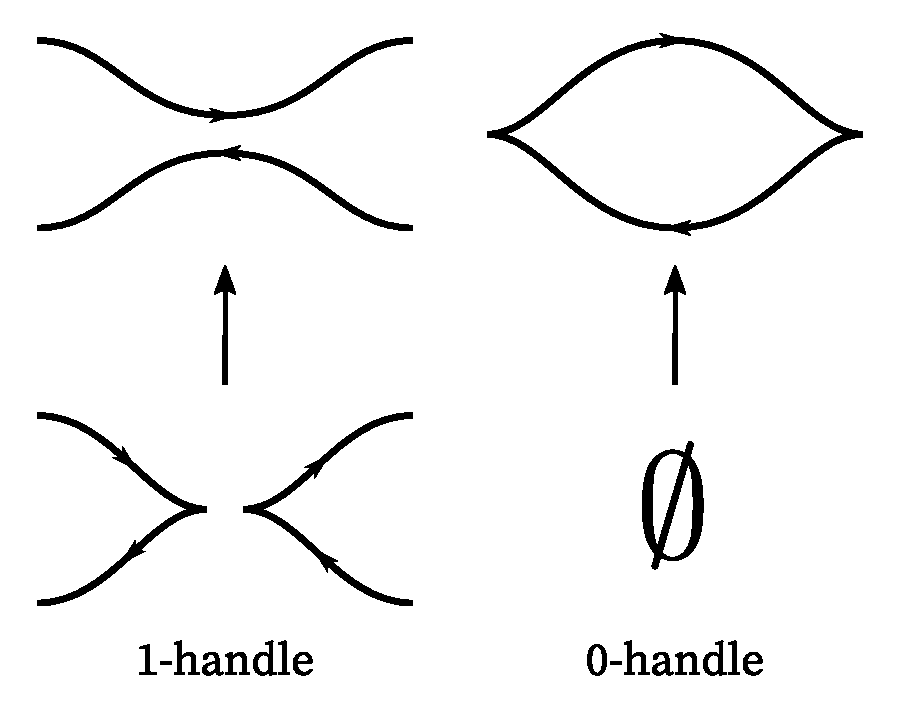
\includegraphics[width=0.4\textwidth]{images/handles.pdf}
    \caption{The handle moves. Note that these moves are one-directional, unlike the Reidemeister moves. The addition of a one-handle is sometimes referred to as a \emph{pinch move}. The addition of a zero-handle corresponds to adding an unlinked unknot with maximal $\tb$ to the diagram.}
    \label{fig:handles}
\end{figure}

We refer to a cobordism that is a result of a sequence of these moves as \textbf{decomposable}. We can represent these cobordisms visually via a sequence along increasing $t$ of front diagrams of Legendrian links, each of which is obtained from the previous by a short (that is, easy to see) sequence of the decomposable moves. For example, Figure~\ref{fig:cobordism-construction} shows a ``movie'' for a decomposable cobordism from a double-stabilized unknot to a Legendrian representative of $m(6_1)$.

\begin{figure}[ht!]
    \centering
    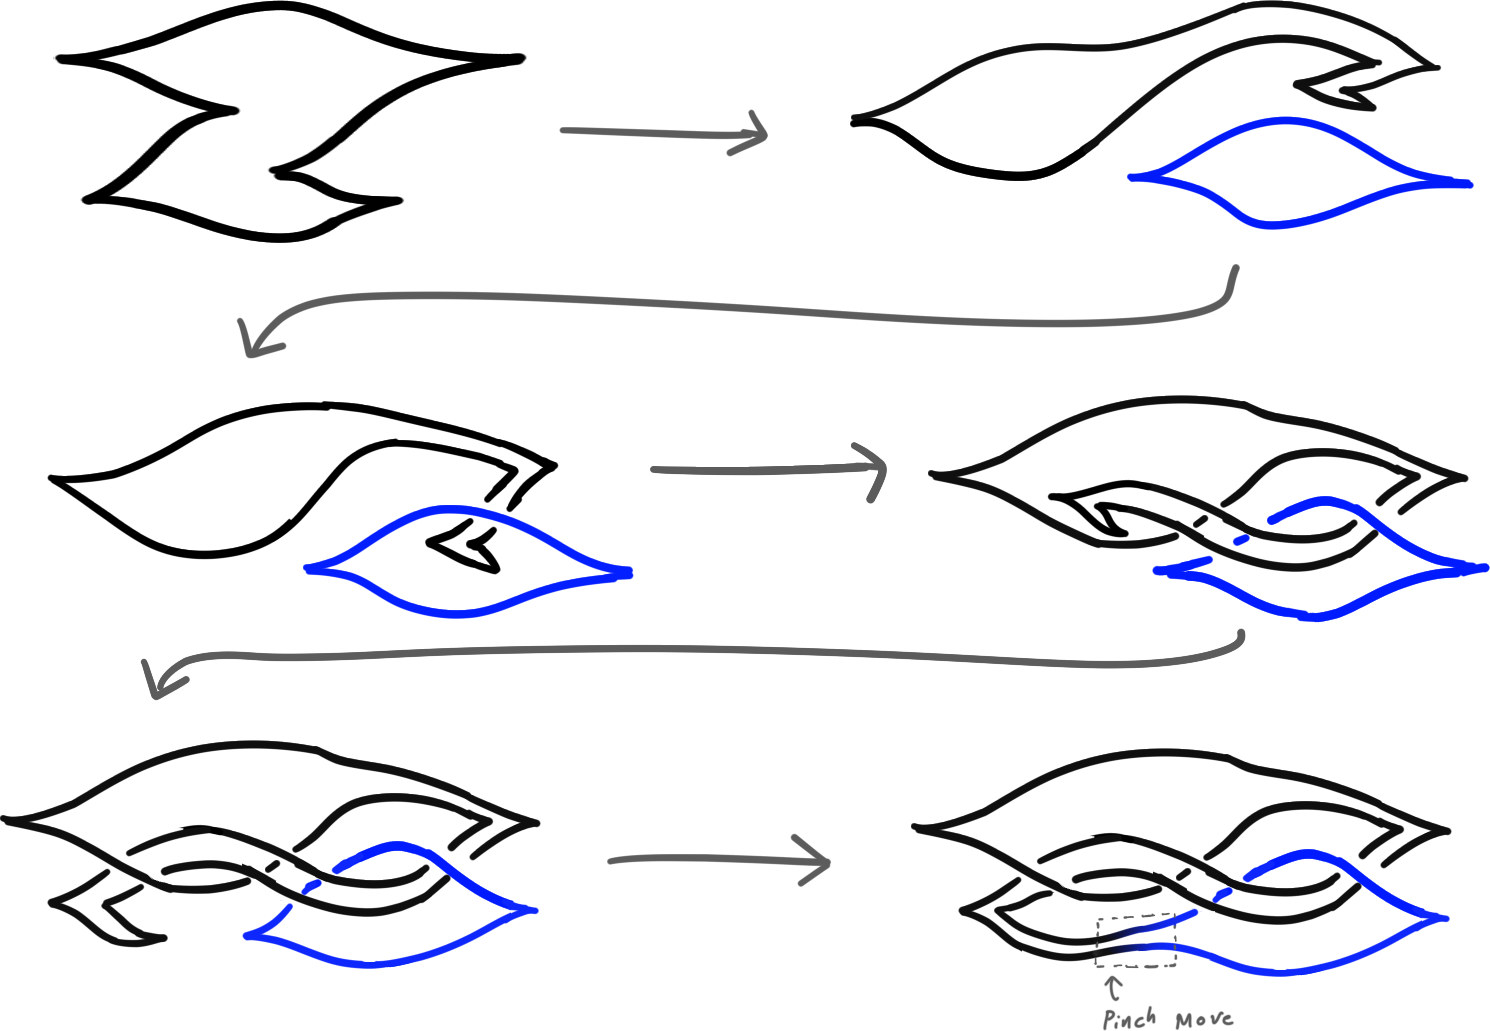
\includegraphics[width=0.5\textwidth]{images/cobordism-construction.png}
    \caption{Constructing a cobordism from the unknot to $m(6_1)$.
    TODO: Make a real nice SVG diagram for this.}%
    \label{fig:cobordism-construction}
\end{figure}

\subsection{Obstructions}

% Be more precise.
It is known that not all Lagrangian cobordisms are decomposable. Moreover, there exist pairs of links $K_-, K_+$ such that a Lagrangian cobordism exists from $K_-$ to $K_+$ but no such decomposable cobordism exists. Specifically, there exists a Lagrangian cobordism from the unknot to the empty set, despite the fact that no decomposable move can give $\emptyset$ from a nonempty Legendrian. It is not known whether this is the case when $K_+ \neq \emptyset$.

% "ends" are removed: cylinder ends.
A number of other obstructions are known to exist. Two of these are particularly easy to state. First, any Lagrangian cobordism yields a topological cobordism if the ends are removed, so any obstructions to the existence of topological cobordisms also obstructs the existence of Lagrangian cobordisms. Second, if there exists a Lagrangian cobordism from $\emptyset$ to $K$, there does not exist a Lagrangian cobordism from $K$ to $\emptyset$ \cite{gromov}. 
% Check this reference.

One obstruction of interest obstructs only decomposable cobordisms. This obstruction is defined in terms of the number of normal rulings, which we will not define here. The theorem is as follows.
TODO: Add reference for information on rulings.
\begin{theorem}
    If $K_-$ has $n$ normal rulings and $K_+$ has $m$ normal rulings with $n > m$, then there is no decomposable Lagrangian cobordism from $K_-$ to $K_+$.
\end{theorem}
Any stabilized knot necessarily has no normal rulings. In light of this fact, this obstruction seems like a promising way to make sense of cobordisms of max-$\tb$ knots. This is true, but only in the case where $K_-$ is maximal.

